\documentclass[a4paper, 10pt] {article}
\usepackage{tikz}
\usepackage[margin = 1cm]{geometry}
\usepackage{xcolor}
\definecolor{customcolor1}{HTML}{abe0f9}
\definecolor{customcolor2}{HTML}{fee4b3}

\title{Data Structure}
\author{Pranto}
\date{\today}

\begin{document}
\maketitle
\section{Graph 3}
Lets Make the Graph of ED task 3.

% 1st
    \vspace{20pt}
    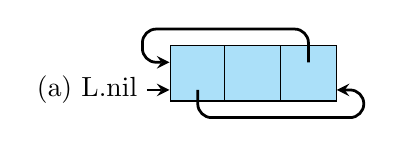
\begin{tikzpicture}
        % Nodes
        \node (a) at (0, 0) {(a) L.nil};
        % \node [draw, rectangle, minimum width = 3cm, minimum height = 1cm] (b) at (3, 0.3) {};
        \node [fill = customcolor1, draw, rectangle, minimum width = 60pt, minimum height = 20pt] (b) at (60pt, 6pt) {};
        % Draw vertical lines to divide the node into three parts
        \draw (b.west) ++(20pt, 10pt) -- ++(0pt, -20pt);
        \draw (b.west) ++(40pt, 10pt) -- ++(0pt, -20pt);
        % Draw the links
        \draw [->, > = stealth, line width = 1pt] (a) -- (b.west |- 0pt, 0pt);      
        \draw [->, > = stealth, line width = 1pt, rounded corners = 5pt] (40pt, 0pt) -- (40pt, -10pt) -- (100pt, -10pt) -- (100pt, 0pt) -- (b.east |- 0pt, 0pt);      
        \draw [->, > = stealth, line width = 1pt, rounded corners = 5pt] (80pt, 10pt) -- (80pt, 22pt) -- (20pt, 22pt) -- (20pt, 10pt) -- (b.west |- 0pt, 10pt);      
          
    \end{tikzpicture}

% 2nd
    \vspace{20pt}
    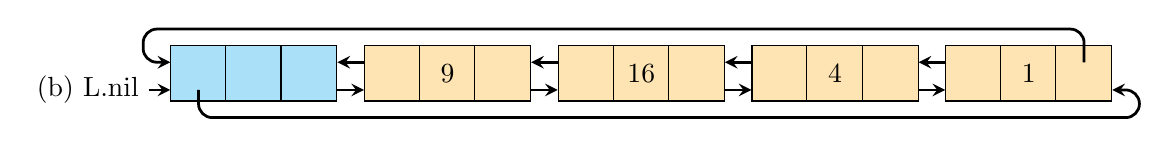
\begin{tikzpicture}
        
        \node (a) at (0, 0) {(b) L.nil};
        \node [fill = customcolor1, draw, rectangle, minimum width = 60pt, minimum height = 20pt] (b) at (60pt, 6pt) {};
        \draw (b.west) ++(20pt, 10pt) -- ++(0pt, -20pt);
        \draw (b.west) ++(40pt, 10pt) -- ++(0pt, -20pt);

        \node [fill = customcolor2, draw, rectangle, minimum width = 60pt, minimum height = 20pt] (c) at (130pt, 6pt) {9};
        \draw (c.west) ++(20pt, 10pt) -- ++(0pt, -20pt);
        \draw (c.west) ++(40pt, 10pt) -- ++(0pt, -20pt);

        \node [fill = customcolor2, draw, rectangle, minimum width = 60pt, minimum height = 20pt] (d) at (200pt, 6pt) {16};
        \draw (d.west) ++(20pt, 10pt) -- ++(0pt, -20pt);
        \draw (d.west) ++(40pt, 10pt) -- ++(0pt, -20pt);

        \node [fill = customcolor2, draw, rectangle, minimum width = 60pt, minimum height = 20pt] (e) at (270pt, 6pt) {4};
        \draw (e.west) ++(20pt, 10pt) -- ++(0pt, -20pt);
        \draw (e.west) ++(40pt, 10pt) -- ++(0pt, -20pt);

        \node [fill = customcolor2, draw, rectangle, minimum width = 60pt, minimum height = 20pt] (f) at (340pt, 6pt) {1};
        \draw (f.west) ++(20pt, 10pt) -- ++(0pt, -20pt);
        \draw (f.west) ++(40pt, 10pt) -- ++(0pt, -20pt);
        
        % Short Direction
        \draw [->, > = stealth, line width = 1pt] (a) -- (b.west |- 0pt, 0pt);  
        \draw [->, > = stealth, line width = 1pt] (b.east |- 0pt, 0pt) -- (c.west |- 0pt, 0pt);  
        \draw [->, > = stealth, line width = 1pt] (c.east |- 0pt, 0pt) -- (d.west |- 0pt, 0pt);  
        \draw [->, > = stealth, line width = 1pt] (d.east |- 0pt, 0pt) -- (e.west |- 0pt, 0pt);  
        \draw [->, > = stealth, line width = 1pt] (e.east |- 0pt, 0pt) -- (f.west |- 0pt, 0pt);  
        \draw [->, > = stealth, line width = 1pt] (c.west |- 0pt, 10pt) -- (b.east |- 0pt, 10pt);  
        \draw [->, > = stealth, line width = 1pt] (d.west |- 0pt, 10pt) -- (c.east |- 0pt, 10pt);  
        \draw [->, > = stealth, line width = 1pt] (e.west |- 0pt, 10pt) -- (d.east |- 0pt, 10pt);  
        \draw [->, > = stealth, line width = 1pt] (f.west |- 0pt, 10pt) -- (e.east |- 0pt, 10pt);  
        
        % Long Direction
        \draw [->, > = stealth, line width = 1pt, rounded corners = 5pt] (40pt, 0pt) -- (40pt, -10pt) -- (380pt, -10pt) -- (380pt, 0pt) -- (f.east |- 0pt, 0pt);      
        \draw [->, > = stealth, line width = 1pt, rounded corners = 5pt] (360pt, 10pt) -- (360pt, 22pt) -- (20pt, 22pt) -- (20pt, 10pt) -- (b.west |- 0pt, 10pt);      
    
    \end{tikzpicture}

% 3rd
    \vspace{20pt}
    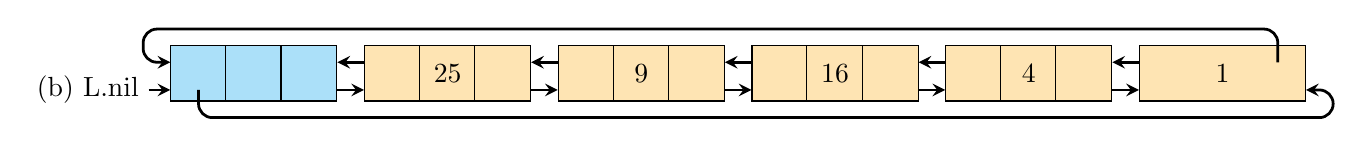
\begin{tikzpicture}

        \node (a) at (0, 0) {(b) L.nil};
        \node [fill = customcolor1, draw, rectangle, minimum width = 60pt, minimum height = 20pt] (b) at (60pt, 6pt) {};
        \draw (b.west) ++(20pt, 10pt) -- ++(0pt, -20pt);
        \draw (b.west) ++(40pt, 10pt) -- ++(0pt, -20pt);

        \node [fill = customcolor2, draw, rectangle, minimum width = 60pt, minimum height = 20pt] (c) at (130pt, 6pt) {25};
        \draw (c.west) ++(20pt, 10pt) -- ++(0pt, -20pt);
        \draw (c.west) ++(40pt, 10pt) -- ++(0pt, -20pt);

        \node [fill = customcolor2, draw, rectangle, minimum width = 60pt, minimum height = 20pt] (d) at (200pt, 6pt) {9};
        \draw (d.west) ++(20pt, 10pt) -- ++(0pt, -20pt);
        \draw (d.west) ++(40pt, 10pt) -- ++(0pt, -20pt);

        \node [fill = customcolor2, draw, rectangle, minimum width = 60pt, minimum height = 20pt] (e) at (270pt, 6pt) {16};
        \draw (e.west) ++(20pt, 10pt) -- ++(0pt, -20pt);
        \draw (e.west) ++(40pt, 10pt) -- ++(0pt, -20pt);

        \node [fill = customcolor2, draw, rectangle, minimum width = 60pt, minimum height = 20pt] (f) at (340pt, 6pt) {4};
        \draw (f.west) ++(20pt, 10pt) -- ++(0pt, -20pt);
        \draw (f.west) ++(40pt, 10pt) -- ++(0pt, -20pt);

        \node [fill = customcolor2, draw, rectangle, minimum width = 60pt, minimum height = 20pt] (g) at (410pt, 6pt) {1};
        \draw (f.west) ++(20pt, 10pt) -- ++(0pt, -20pt);
        \draw (f.west) ++(40pt, 10pt) -- ++(0pt, -20pt);
        
        % Short Direction
        \draw [->, > = stealth, line width = 1pt] (a) -- (b.west |- 0pt, 0pt);  
        \draw [->, > = stealth, line width = 1pt] (b.east |- 0pt, 0pt) -- (c.west |- 0pt, 0pt);  
        \draw [->, > = stealth, line width = 1pt] (c.east |- 0pt, 0pt) -- (d.west |- 0pt, 0pt);  
        \draw [->, > = stealth, line width = 1pt] (d.east |- 0pt, 0pt) -- (e.west |- 0pt, 0pt);  
        \draw [->, > = stealth, line width = 1pt] (e.east |- 0pt, 0pt) -- (f.west |- 0pt, 0pt);  
        \draw [->, > = stealth, line width = 1pt] (f.east |- 0pt, 0pt) -- (g.west |- 0pt, 0pt);  
        \draw [->, > = stealth, line width = 1pt] (c.west |- 0pt, 10pt) -- (b.east |- 0pt, 10pt);  
        \draw [->, > = stealth, line width = 1pt] (d.west |- 0pt, 10pt) -- (c.east |- 0pt, 10pt);  
        \draw [->, > = stealth, line width = 1pt] (e.west |- 0pt, 10pt) -- (d.east |- 0pt, 10pt);  
        \draw [->, > = stealth, line width = 1pt] (f.west |- 0pt, 10pt) -- (e.east |- 0pt, 10pt);  
        \draw [->, > = stealth, line width = 1pt] (g.west |- 0pt, 10pt) -- (f.east |- 0pt, 10pt);  
        
        % Long Direction
        \draw [->, > = stealth, line width = 1pt, rounded corners = 5pt] (40pt, 0pt) -- (40pt, -10pt) -- (450pt, -10pt) -- (450pt, 0pt) -- (g.east |- 0pt, 0pt);      
        \draw [->, > = stealth, line width = 1pt, rounded corners = 5pt] (430pt, 10pt) -- (430pt, 22pt) -- (20pt, 22pt) -- (20pt, 10pt) -- (b.west |- 0pt, 10pt);      

    \end{tikzpicture}

% 4th
    \vspace{20pt}
    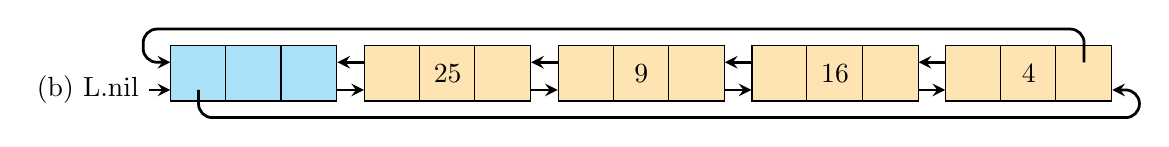
\begin{tikzpicture}

        \node (a) at (0, 0) {(b) L.nil};
        \node [fill = customcolor1, draw, rectangle, minimum width = 60pt, minimum height = 20pt] (b) at (60pt, 6pt) {};
        \draw (b.west) ++(20pt, 10pt) -- ++(0pt, -20pt);
        \draw (b.west) ++(40pt, 10pt) -- ++(0pt, -20pt);

        \node [fill = customcolor2, draw, rectangle, minimum width = 60pt, minimum height = 20pt] (c) at (130pt, 6pt) {25};
        \draw (c.west) ++(20pt, 10pt) -- ++(0pt, -20pt);
        \draw (c.west) ++(40pt, 10pt) -- ++(0pt, -20pt);

        \node [fill = customcolor2, draw, rectangle, minimum width = 60pt, minimum height = 20pt] (d) at (200pt, 6pt) {9};
        \draw (d.west) ++(20pt, 10pt) -- ++(0pt, -20pt);
        \draw (d.west) ++(40pt, 10pt) -- ++(0pt, -20pt);

        \node [fill = customcolor2, draw, rectangle, minimum width = 60pt, minimum height = 20pt] (e) at (270pt, 6pt) {16};
        \draw (e.west) ++(20pt, 10pt) -- ++(0pt, -20pt);
        \draw (e.west) ++(40pt, 10pt) -- ++(0pt, -20pt);

        \node [fill = customcolor2, draw, rectangle, minimum width = 60pt, minimum height = 20pt] (f) at (340pt, 6pt) {4};
        \draw (f.west) ++(20pt, 10pt) -- ++(0pt, -20pt);
        \draw (f.west) ++(40pt, 10pt) -- ++(0pt, -20pt);
        
        % Short Direction
        \draw [->, > = stealth, line width = 1pt] (a) -- (b.west |- 0pt, 0pt);  
        \draw [->, > = stealth, line width = 1pt] (b.east |- 0pt, 0pt) -- (c.west |- 0pt, 0pt);  
        \draw [->, > = stealth, line width = 1pt] (c.east |- 0pt, 0pt) -- (d.west |- 0pt, 0pt);  
        \draw [->, > = stealth, line width = 1pt] (d.east |- 0pt, 0pt) -- (e.west |- 0pt, 0pt);  
        \draw [->, > = stealth, line width = 1pt] (e.east |- 0pt, 0pt) -- (f.west |- 0pt, 0pt);  
        \draw [->, > = stealth, line width = 1pt] (c.west |- 0pt, 10pt) -- (b.east |- 0pt, 10pt);  
        \draw [->, > = stealth, line width = 1pt] (d.west |- 0pt, 10pt) -- (c.east |- 0pt, 10pt);  
        \draw [->, > = stealth, line width = 1pt] (e.west |- 0pt, 10pt) -- (d.east |- 0pt, 10pt);  
        \draw [->, > = stealth, line width = 1pt] (f.west |- 0pt, 10pt) -- (e.east |- 0pt, 10pt);  
        
        % Long Direction
        \draw [->, > = stealth, line width = 1pt, rounded corners = 5pt] (40pt, 0pt) -- (40pt, -10pt) -- (380pt, -10pt) -- (380pt, 0pt) -- (f.east |- 0pt, 0pt);      
        \draw [->, > = stealth, line width = 1pt, rounded corners = 5pt] (360pt, 10pt) -- (360pt, 22pt) -- (20pt, 22pt) -- (20pt, 10pt) -- (b.west |- 0pt, 10pt);      

    \end{tikzpicture}

% 5th
    \vspace{20pt}
    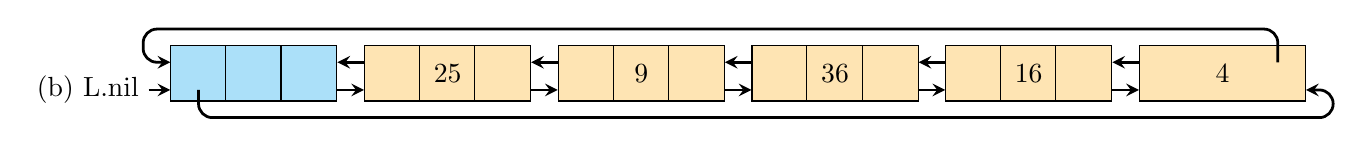
\begin{tikzpicture}

        \node (a) at (0, 0) {(b) L.nil};
        \node [fill = customcolor1, draw, rectangle, minimum width = 60pt, minimum height = 20pt] (b) at (60pt, 6pt) {};
        \draw (b.west) ++(20pt, 10pt) -- ++(0pt, -20pt);
        \draw (b.west) ++(40pt, 10pt) -- ++(0pt, -20pt);

        \node [fill = customcolor2, draw, rectangle, minimum width = 60pt, minimum height = 20pt] (c) at (130pt, 6pt) {25};
        \draw (c.west) ++(20pt, 10pt) -- ++(0pt, -20pt);
        \draw (c.west) ++(40pt, 10pt) -- ++(0pt, -20pt);

        \node [fill = customcolor2, draw, rectangle, minimum width = 60pt, minimum height = 20pt] (d) at (200pt, 6pt) {9};
        \draw (d.west) ++(20pt, 10pt) -- ++(0pt, -20pt);
        \draw (d.west) ++(40pt, 10pt) -- ++(0pt, -20pt);

        \node [fill = customcolor2, draw, rectangle, minimum width = 60pt, minimum height = 20pt] (e) at (270pt, 6pt) {36};
        \draw (e.west) ++(20pt, 10pt) -- ++(0pt, -20pt);
        \draw (e.west) ++(40pt, 10pt) -- ++(0pt, -20pt);

        \node [fill = customcolor2, draw, rectangle, minimum width = 60pt, minimum height = 20pt] (f) at (340pt, 6pt) {16};
        \draw (f.west) ++(20pt, 10pt) -- ++(0pt, -20pt);
        \draw (f.west) ++(40pt, 10pt) -- ++(0pt, -20pt);

        \node [fill = customcolor2, draw, rectangle, minimum width = 60pt, minimum height = 20pt] (g) at (410pt, 6pt) {4};
        \draw (f.west) ++(20pt, 10pt) -- ++(0pt, -20pt);
        \draw (f.west) ++(40pt, 10pt) -- ++(0pt, -20pt);
        
        % Short Direction
        \draw [->, > = stealth, line width = 1pt] (a) -- (b.west |- 0pt, 0pt);  
        \draw [->, > = stealth, line width = 1pt] (b.east |- 0pt, 0pt) -- (c.west |- 0pt, 0pt);  
        \draw [->, > = stealth, line width = 1pt] (c.east |- 0pt, 0pt) -- (d.west |- 0pt, 0pt);  
        \draw [->, > = stealth, line width = 1pt] (d.east |- 0pt, 0pt) -- (e.west |- 0pt, 0pt);  
        \draw [->, > = stealth, line width = 1pt] (e.east |- 0pt, 0pt) -- (f.west |- 0pt, 0pt);  
        \draw [->, > = stealth, line width = 1pt] (f.east |- 0pt, 0pt) -- (g.west |- 0pt, 0pt);  
        \draw [->, > = stealth, line width = 1pt] (c.west |- 0pt, 10pt) -- (b.east |- 0pt, 10pt);  
        \draw [->, > = stealth, line width = 1pt] (d.west |- 0pt, 10pt) -- (c.east |- 0pt, 10pt);  
        \draw [->, > = stealth, line width = 1pt] (e.west |- 0pt, 10pt) -- (d.east |- 0pt, 10pt);  
        \draw [->, > = stealth, line width = 1pt] (f.west |- 0pt, 10pt) -- (e.east |- 0pt, 10pt);  
        \draw [->, > = stealth, line width = 1pt] (g.west |- 0pt, 10pt) -- (f.east |- 0pt, 10pt);  
        
        % Long Direction
        \draw [->, > = stealth, line width = 1pt, rounded corners = 5pt] (40pt, 0pt) -- (40pt, -10pt) -- (450pt, -10pt) -- (450pt, 0pt) -- (g.east |- 0pt, 0pt);      
        \draw [->, > = stealth, line width = 1pt, rounded corners = 5pt] (430pt, 10pt) -- (430pt, 22pt) -- (20pt, 22pt) -- (20pt, 10pt) -- (b.west |- 0pt, 10pt);      

    \end{tikzpicture}
\end{document}